% % % % % % % % % % % % % % % % % % % % % % % % % % % % % % % % % % % % % % % % % % % %
%                                                                                     %
% Short Sectioned Assignment LaTeX Template Version 1.0 (5/5/12)                      %
% This template has been downloaded from: http://www.LaTeXTemplates.com               %
%                                                                                     %
% Original author:  Frits Wenneker (http://www.howtotex.com)                          %
%                                                                                     %
% Modified by: Fco Javier Sueza Rodríguez (fcosueza@disroot.org)                      %
%                                                                                     %
% Changes:                                                                            %
%	    - Custom Chapters, Sections and Subsections (titlesec package)                %
%           - Document type scrbook (oneside)                                         %
%           - Use babel-lang-spanish package and marvosym                             %
%           - Use hyperref, enumitem, tcolorbox and glossaries packages               %
%           - Use Time New Roman (mathptmx), Helvetic and Courier fonts               %
%                                                                                     %
% License: CC BY-NC-SA 3.0 (http://creativecommons.org/licenses/by-nc-sa/3.0/)        %
%                                                                                     %
% % % % % % % % % % % % % % % % % % % % % % % % % % % % % % % % % % % % % % % % % % % %

%-----------------------------------------------%
%	              Packages                  %
%-----------------------------------------------%

\documentclass[paper=a4, fontsize=11pt, oneside]{scrbook}

% ---- Text Input/Output ----- %

\usepackage[T1]{fontenc}
\usepackage[utf8]{inputenc}
\usepackage{mathptmx}
\usepackage[scaled=.92]{helvet}
\usepackage{courier}
\usepackage[indent=12pt]{parskip}

\usepackage{geometry}
\geometry{verbose,tmargin=3cm,bmargin=3cm,lmargin=2.6cm,rmargin=2.6cm}

% ---- Language ----- %

\usepackage[spanish]{babel}
\usepackage{marvosym}

% ---- Another packages ---- %

\usepackage{amsmath,amsfonts,amsthm}
\usepackage{graphics,graphicx}
\usepackage{titlesec}
\usepackage{fancyhdr}
\usepackage{tcolorbox}
\usepackage{hyperref}
\usepackage{enumitem}
\usepackage[automake]{glossaries}

%--------------------------------------------------------------------%
%                      Customizing Document                          %
%--------------------------------------------------------------------%


% ----------- Custom Chapters, Sections and Subsections -------------- %

\titleformat{\chapter}[display]
			{\bfseries\Huge}
			{Tema \ \thechapter} {0.5ex}
			{\vspace{1ex}\centering}

\titleformat{\section}[hang]
			{\bfseries\Large}
			{\thesection}{0.5em}{}

\titleformat{\subsection}[hang]
			{\bfseries\large}
			{\thesubsection}{0.5em}{}

\titleformat{\subsubsection}[hang]
			{\bfseries\large}
			{\thesubsubsection}{0.5em}{}

\hypersetup{
    colorlinks=true,
    linkcolor=black,
    urlcolor=magenta
}

% ------------------- Custom heaaders and footers ------------------- %

\pagestyle{fancyplain}

\fancyhead[]{}
\fancyfoot[L]{}
\fancyfoot[C]{}
\fancyfoot[R]{\thepage}

\renewcommand{\headrulewidth}{0pt} % Remove header underlines
\renewcommand{\footrulewidth}{0pt} % Remove footer underlines

\setlength{\headheight}{13.6pt} % Customize the height of the header

% --------- Numbering equations, figures and tables ----------------- %

\numberwithin{equation}{section} % Number equations within sections
\numberwithin{figure}{section} % Number figures within sections
\numberwithin{table}{section} % Number tables within sections

% ------------------------ New Commands ----------------------------- %

\newcommand{\horrule}[1]{\rule{\linewidth}{#1}} % Create horizontal rule command


%----------------------------------------------------------------------------------------
%	TÍTULO Y DATOS DEL ALUMNO
%----------------------------------------------------------------------------------------

\title{
\vspace{10ex}
\normalfont \normalsize
\huge \textbf{Tarea 5: CRO + WPO. Optimizando mi Web}
}
\author{Francisco Javier Sueza Rodríguez}
\date{\normalsize\today}

%----------------------------------------------------------------------------------------
%                                     DOCUMENTO
%----------------------------------------------------------------------------------------
\begin{document}

\maketitle

\thispagestyle{empty}

\vspace{65ex}

\begin{center}
    \begin{tabular}{l l}
        \textbf{Centro}: & IES Aguadulce \\
        \textbf{Ciclo Formativo}: & Desarrollo Aplicaciones Web (Distancia)\\
        \textbf{Asignatura}: & Horas de Libre Configuración\\
        \textbf{Tema}: & Tema 5 - CRO + WPO. Optimizando mi Web`\\
    \end{tabular}
\end{center}

\newpage

\tableofcontents

\vspace{15ex}

\listoffigures

\newpage

\section{Ejercicio 1: Glosario de Términos}
Realiza un \textbf{glosario} de los siguientes términos empleados en la UT, explicando el significado de cada uno de ellos, no debe ser una definición muy técnica si no algo que pueda entender una persona sin amplios conocimientos del tema.

\begin{itemize}
    \item ROI
    \item CTA
    \item CRO
    \item WPO
\end{itemize}

\subsection{Solución}
En este ejercicio vamos a realizar un \textbf{glosario} con varios términos relacionados con la optimización web. Estos términos son:

\begin{itemize}
    \item \textbf{ROI} (Return Of Investment): el retorno de la inversión es una de las principales métricas en marketing y sirve para calcular si una campaña de marketing o acción concreta está siendo rentable.

    \item \textbf{CTA} (Call To Action): la llamada a la acción es una técnica que emplea imágenes, textos y otros elementos para incitar a los usuarios a realizar una acción determinada, como comprar un producto, darse de alta en una web, realizar una suscripción, etc...

    \item \textbf{CRO} (Conversión Rate Optmization): la \textbf{optimización del ratio de conversión} son diferentes técnicas que se emplean para optimizar una web y que aumente la cantidad de acciones que realizan los usuarios y que nosotros deseamos que realicen, como por ejemplo, suscribirse al correo de la web, darse de alta, comprar algún producto, etc...

    \item \textbf{WPO} (Web Performance Optimization): en este casi, la \textbf{optimización del rendimiento Web} son un grupo de técnicas enfocados en optimizar nuestra web y mejorar los tiempos de carga de ésta, así como la accesibilidad y la usabilidad, mejorando la experiencia de usuario.
\end{itemize}

\section{Ejercicio 2:  Instala la extensión de Google Chrome Lighthouse}
\begin{itemize}
    \item
    Desde esta URL podrás instalar la extensión a Google Chrome: \href{https://chromewebstore.google.com/detail/lighthouse/blipmdconlkpinefehnmjammfjpmpbjk?hl=es&pli=1}{LightHouse}

    \item Selecciona una página web de un \textbf{supermercado} genera el archivo de auditoria con Lighthouse. Hazlo primero con Chrome de manera normal y después desde ventana de incógnito verás la diferencia de puntuación.

    \item ¿Qué puntuación asigna al sitio web que estás utilizando?

    \item Explica al menos 3 sugerencias de mejora que nos sugiera el informe.
\end{itemize}

\subsection{Solución}
En esta actividad se va a realizar la instalación de \textbf{Lighthouse} en Google Chrome y se va a realizar el análisis de una web de un supermercado, explicando las métricas que nos muestra el informe, la puntuación que obtiene el sitio web analizado y 3 sugerencias de mejora que nos haga Lighthouse.

\begin{itemize}
    \item En primer lugar hemos realizado la \textbf{instalación} de Lighthouse. Para ello hemos seguido el enlace que se nos muestra en el enunciado y hemos pulsado en el botón \textbf{Añadir a Chrome}. En la siguiente captura, podemos ver con se ha realizado la instalación en el navegado Google Chrome.

    \begin{figure}[H]
        \centering
        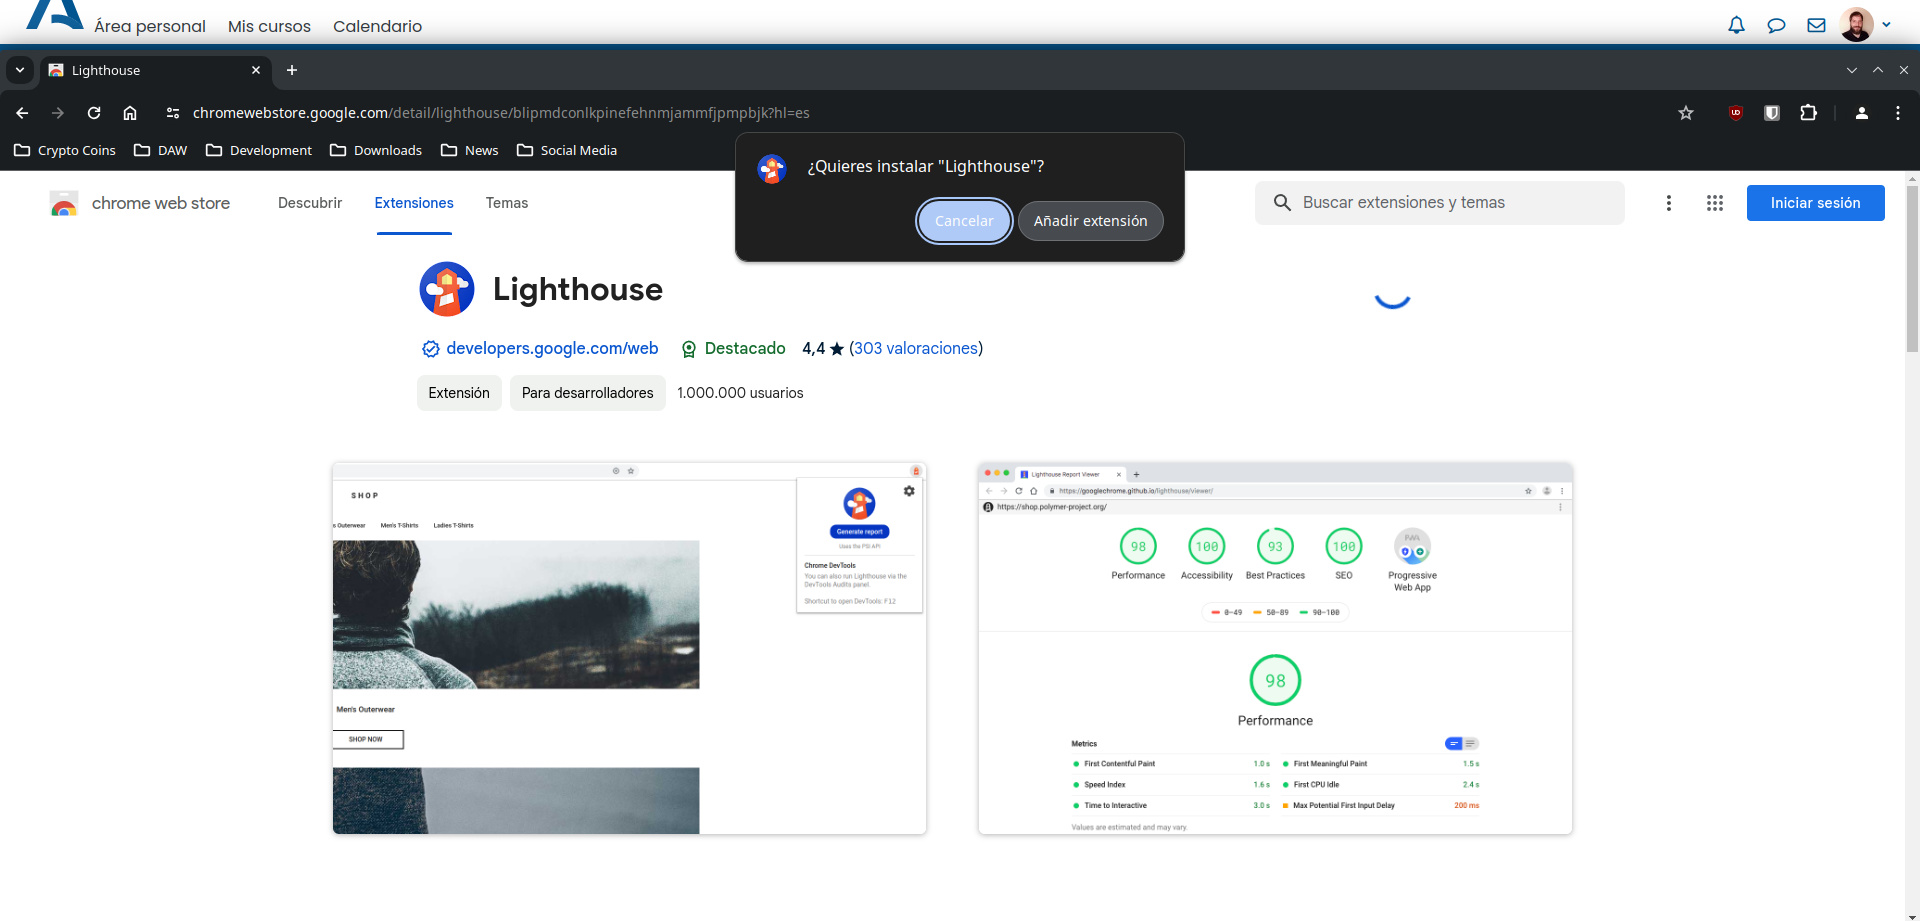
\includegraphics[scale=0.27]{lh-install.png}
        \caption{Instalación de Lighthouse en Google Chrome}
    \end{figure}

    \item En el siguiente paso se han realizado dos análisis sobre el la web del supermercado \href{https://www.mercadona.es/}{Mercadona}. El primer análisis se ha realizado de forma normal, como podemos ver en la siguiente captura de pantalla.

    \begin{figure}[H]
        \centering
        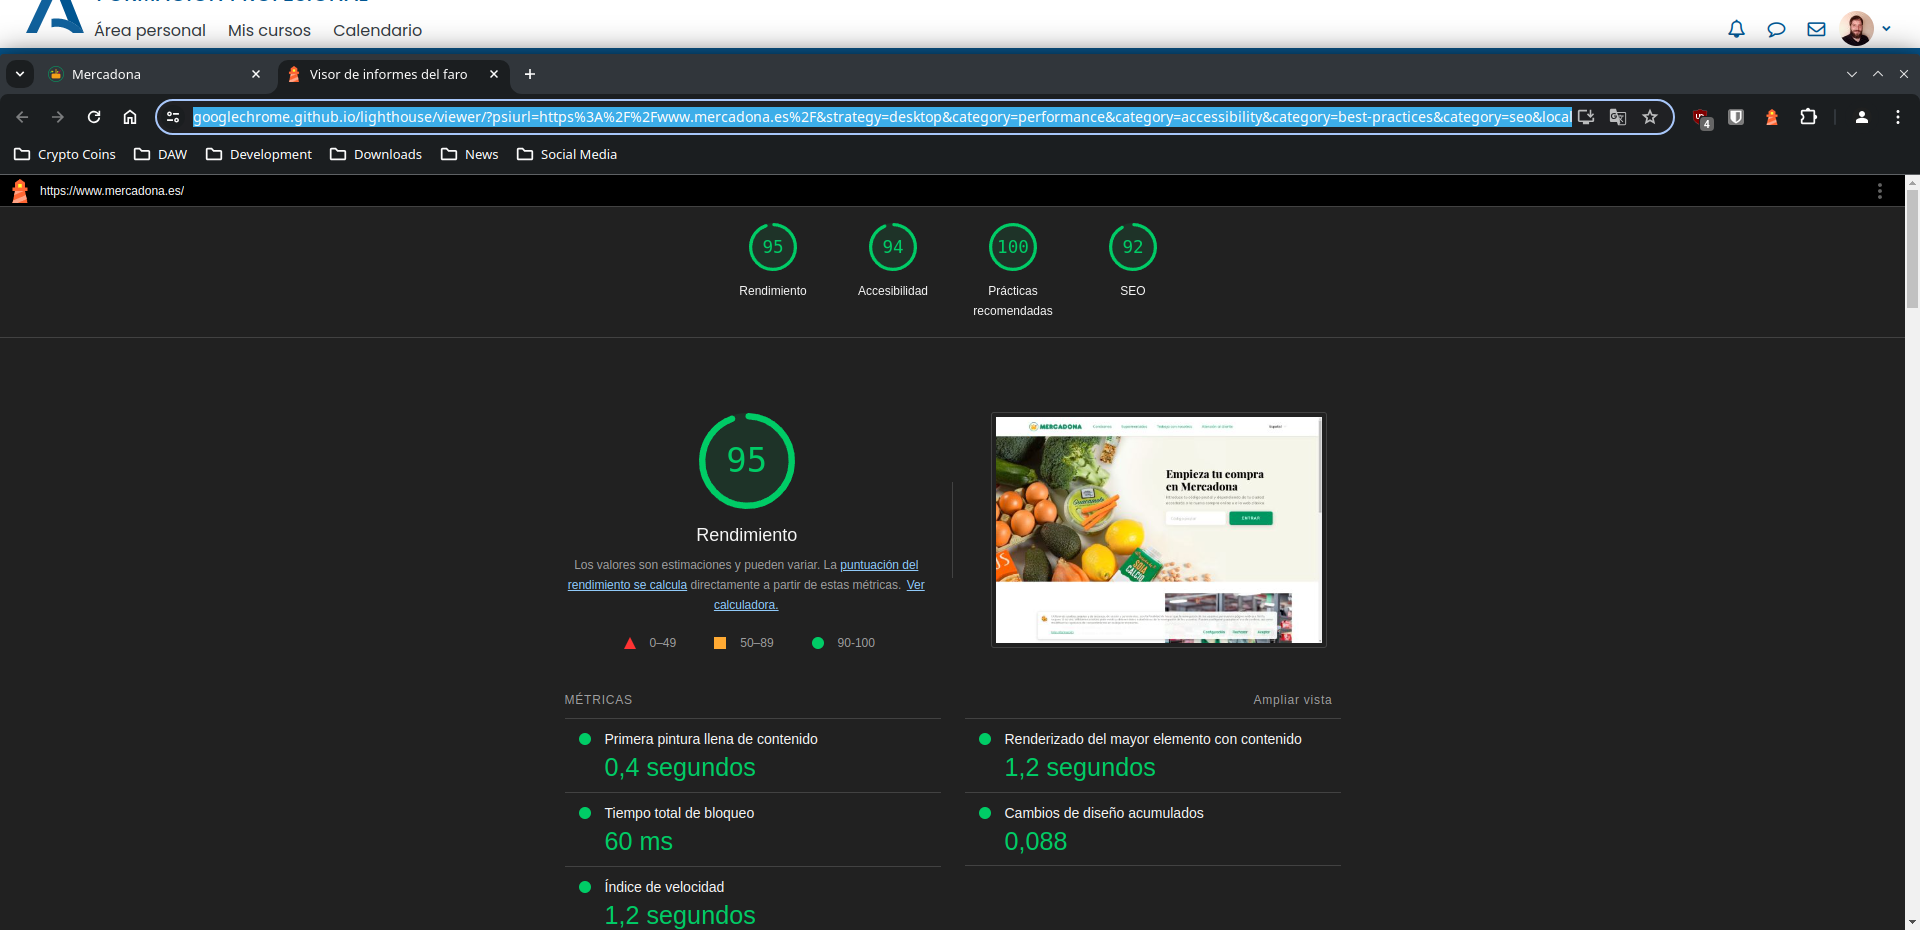
\includegraphics[scale=0.27]{lh-merca-1.png}
        \caption{Análisis de la web de Mercadona en modo normal}
    \end{figure}

    \item El siguiente paso ha sido realizar el mismo análisis, pero en este caso, se ha realizado con el navegador en \textbf{modo incógnito}.
\end{itemize}
% Bibliography

%\newpage
%\bibliography{citas}
%\bibliographystyle{unsrt}

\end{document}